
\documentclass[12pt,epsfig,color,russian]{article}
\usepackage[russian]{babel}
\usepackage{epsfig}
\usepackage{color}

\topmargin=0cm
\hoffset -30mm
\voffset -12mm
\setlength{\unitlength}{1mm}
\parindent=10mm
\textheight=250mm
\textwidth=185mm
\pagestyle{empty}

\begin{document}
\sf\Large
\centerline{\LARGE\bf Молекулярные явления в жидкостях}

Уравнение Ван-дер-Ваальса описывает не только реальные газы, но и жидкости. При температуре $<$ критической различие газ--жидкость ста\-но\-вит\-ся большим. Плотность жидкости и ее насыщенных паров отличается в тысячи раз. $\exists$ растянутые жидкости $\Rightarrow\exists$ прочность на разрыв.\\
 \begin{picture}(185,60)(0,0)
 %\put(0,0){\framebox(185,60)[b]{}}
 \put(0,0){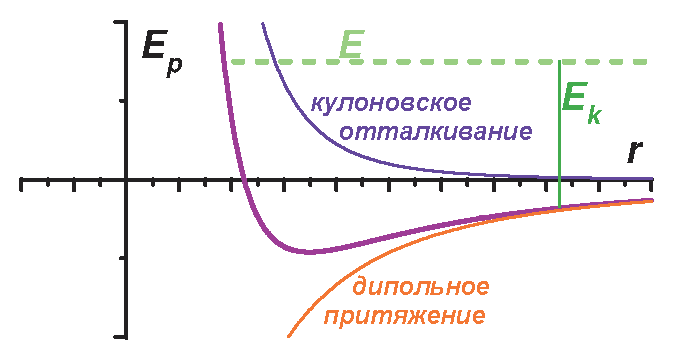
\includegraphics{GP013F01.eps}}
 \put(125,55){\makebox(0,0)[tl]{\parbox{65mm}{
 В газе кинетическая энер\-гия молекул $E_k\gg$ чем энер\-гия связи $\Rightarrow$ молекулы свободно дви\-жут\-ся между столк\-но\-ве\-ни\-я\-ми, и длина свободного пробега $\lambda\gg$ размера молекул.
 }}}
 \end{picture}\\[5mm]
 Энергии не хватает, чтобы преодолеть притяжение $\Rightarrow$ жидкость занимает конечный объем.
 В жидкости расстояния между молекулами срав\-ни\-мы с их размерами $\Rightarrow$ вза\-и\-мо\-дей\-ствие $\gg$ чем в газах. Каждая молекула взаимодействует с \underline{\bf несколькими} соседними $\Rightarrow E_p=$ сумме потенциалов:\\
 \begin{picture}(185,110)(0,0)
 %\put(0,0){\framebox(185,110)[b]{}}
 \put(20,0){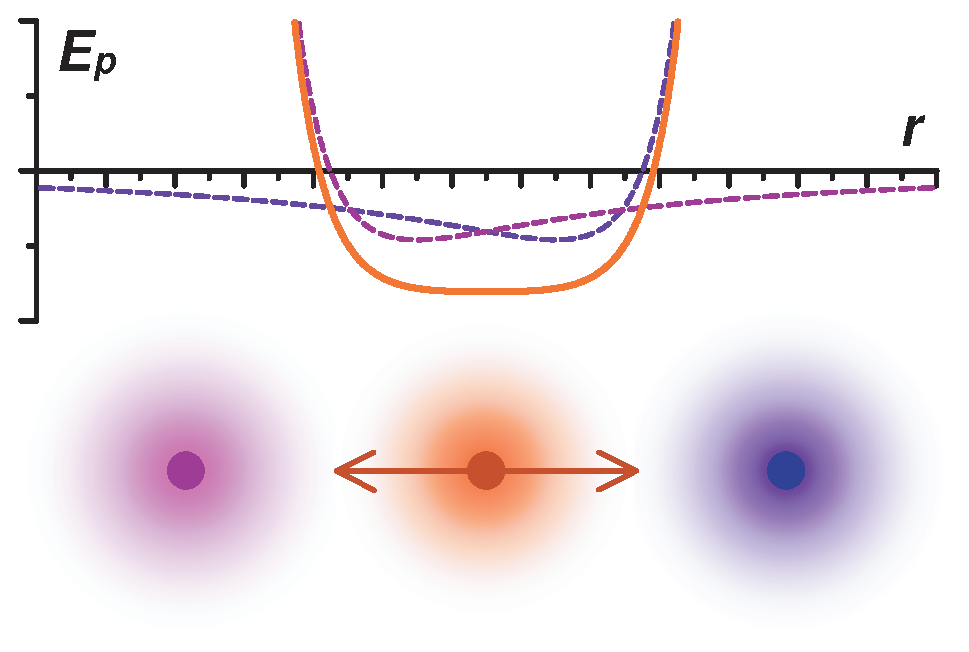
\includegraphics{GP013F02.eps}}
 \end{picture}
 \newpage
 График для $E_p$ становится периодическим (причем учитывать надо, конечно, не ВСЕ молекулы, а только {\bf ближний порядок}:\\
 \begin{picture}(185,100)(0,0)
 %\put(0,0){\framebox(185,100)[b]{}}
 \put(20,0){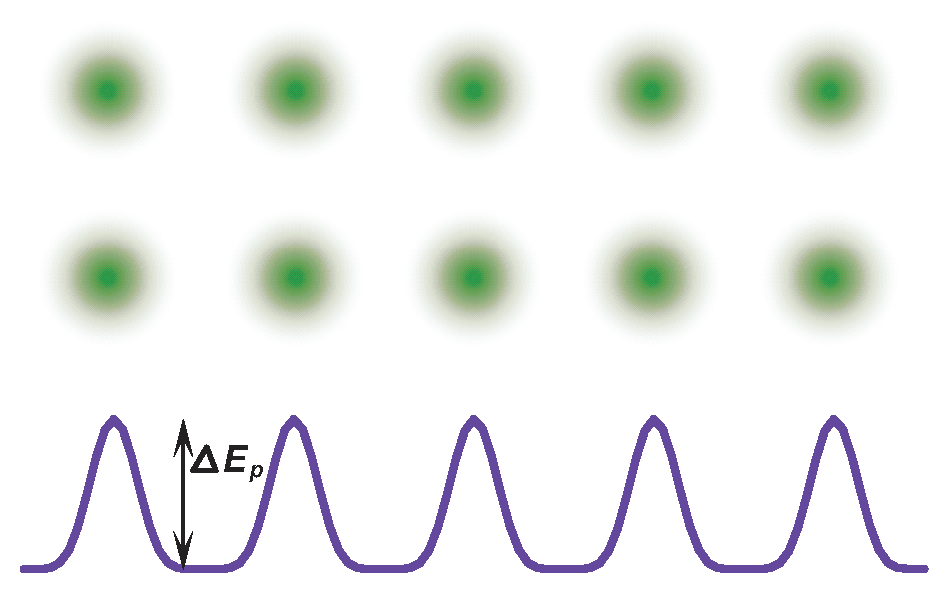
\includegraphics{GP013F03.eps}}
 \end{picture}\\


В тв.теле каждый атом сидит в своей потенциальной яме и не в силах оттуда выбраться, а может там только колебаться.  У жидкости более рыхлая структура, есть свободные места -- ``дырки''.
 Поскольку $\frac12kT$ не намного < глубины ямы, то часть времени молекула ведет оседлый образ жизни, а потом из-за флуктуаций (распределение Максвелла!) переска\-ки\-ва\-ет в соседнюю ямку $\Rightarrow$ в жидкости возможна {\bf диффузия}.
Она $\ll$ чем в газе, но $\gg$ чем в тв.теле.
Только некоторые (самые быстрые) молекулы способны вырваться $\Rightarrow$ {\bf испарение}.\\
 \begin{picture}(185,50)(0,0)
 %\put(0,0){\framebox(185,50)[b]{}}
 \put(108,0){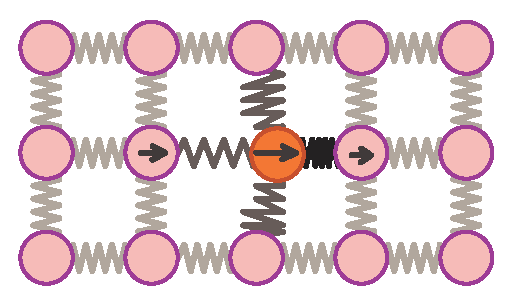
\includegraphics{GP013F04.eps}}
 \put(0,45){\makebox(0,0)[tl]{\parbox{103mm}{
{\bf Трение} в газе: перенос количества движения из слоя в слой за счет перелета молекул на длину свободного пробега. В жидкости $\exists$ еще один механизм: фононный. Шарик не только толкает правого соседа, но и тащит левого.
}}}
 \end{picture}\\
Возникает волна, которая катится по жидкости и несет импульс.\\
 \begin{picture}(185,50)(0,0)
 %\put(0,0){\framebox(185,50)[b]{}}
 \put(108,0){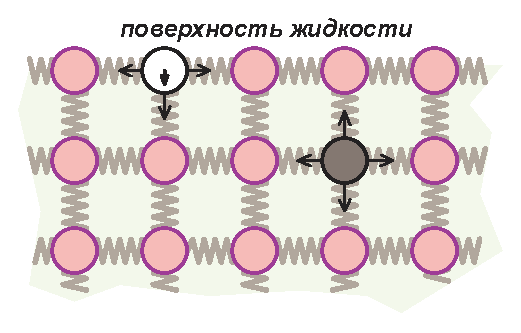
\includegraphics{GP013F05.eps}}
 \put(0,45){\makebox(0,0)[tl]{\parbox{103mm}{
Молекулы на {\bf поверхности}: ``соседей'' сверху НЕТ $\Rightarrow$ силы нескомпенсированы $\Rightarrow \exists$ результирующая $\neq 0$, направленная НОРМАЛЬНО к поверхности.\\ На поверхности {\em как бы} есть {\em как бы} пленка, которая хочет сжаться.
}}}
 \end{picture}\\
Явление {\bf поверхностного натяжения}. Жидкость $\rightarrow$ к сферической форме (минимальная поверхность): капли, пена, пузыри,...\\
 \begin{picture}(185,40)(0,0)
 %\put(0,0){\framebox(185,40)[b]{}}
 \put(0,0){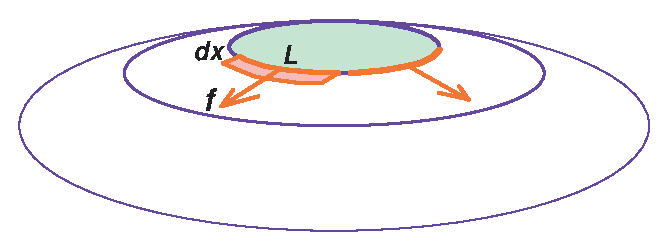
\includegraphics{GP013F06.eps}}
 \put(110,38){\makebox(0,0)[tl]{\parbox{75mm}{
Чтобы удержать пленку от стя\-гивания, нужна сила по ка\-са\-тель\-ной к поверхности, про\-пор\-ци\-о\-наль\-ная границе:\vspace{-5mm}
\begin{displaymath}
f=\alpha\;L
\end{displaymath}
}}}
 \end{picture}\\
Коэффициент поверхностного натяжения $\alpha=f/L$ [дин/см] убывает с ростом температуры. При $T\rightarrow T_k \;\;\;\alpha\rightarrow0$. Вода (н.у.): $\alpha=73$ дин/см.\\
Если сдвинуть границу пленки $L$ на расстояние $dx$, то совершится работа $dA=f\;dx=\alpha\;L\;dx=\alpha\;dS$ (где $dS$ -- увеличение площади пленки). Эта работа идет на увеличение внутренней энергии $E$. $\Rightarrow$ еще одно определение коэф-та $\alpha$: $\alpha=dE/dS$.\\
 \begin{picture}(185,28)(0,0)
 %\put(0,0){\framebox(185,30)[b]{}}
 \put(95,0){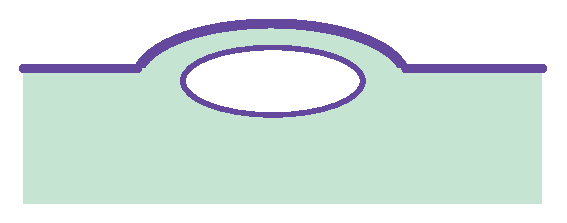
\includegraphics{GP013F07.eps}}
 \put(0,22){\makebox(0,0)[tl]{\parbox{90mm}{
 Всплывающий пузырь не может прорвать пленку на поверхности воды $\Rightarrow$ образование пены.
}}}
 \end{picture}\\
 У мыльной воды $\alpha$ меньше, но вязкость больше, $\Rightarrow$ она медленнее вытекает из слоя между пузырем и поверхностью, и пена дольше остается.\\
  \begin{picture}(185,45)(0,0)
 %\put(0,0){\framebox(185,45)[b]{}}
 \put(0,0){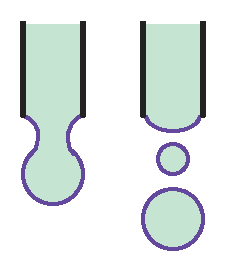
\includegraphics{GP013F08.eps}}
 \put(40,40){\makebox(0,0)[tl]{\parbox{145mm}{
 Вытекающая вода образует капли, которые после отрыва принимают сферическую форму. Если давление в трубке недостаточно, то капля вообще не сможет оторваться! (Палатка пропускает воздух, а воду -- нет). Дело в соотношении диаметра трубки, кривизны капли, и т. д.
}}}
 \end{picture}\\
 \begin{picture}(185,60)(0,0)
 %\put(0,0){\framebox(185,60)[b]{}}
 \put(140,0){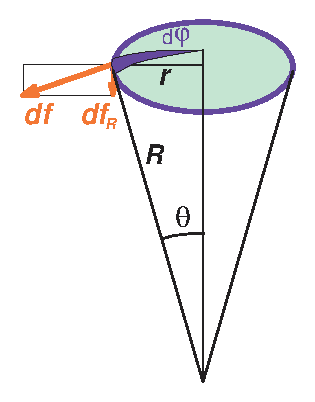
\includegraphics{GP013F09.eps}}
 \put(0,60){\makebox(0,0)[tl]{\parbox{135mm}{
 Рассмотрим кусочек сферической поверхности пу\-зырь\-ка с радиусом $R$. Если выделить маленькую дугу, соответствующую углу $d\varphi$, то ее длина будет $r\,d\varphi$, и
 }}}
 \put(0,37){\makebox(0,0)[tl]{\parbox{155mm}{
 сила, направленная по касательной к поверхности и $\bot$ этой дуге: $df=\alpha\,r\,d\varphi$, а ее вертикальная со\-став\-ля\-ю\-щая: $df_1=\alpha\,r\,\sin\theta\,d\varphi$. Если теперь просуммировать все силы $df_1$ от каждой из дуг, на которые разбивается граница нашего выбранного кусочка (т.е., говоря по-русски, проинтегрировать
}}}
 \end{picture}\\
  по $\varphi$, то получим суммарную силу, с которой наш кусочек поверхности площадью $\pi r^2$ давит вниз на находящуюся под ним жидкость:
  \begin{displaymath}
  f_1=\int\limits_0^{2\pi}\alpha\,r\,\sin\theta\,d\varphi=2\pi\,\alpha\,r\,\sin\theta=
  2\alpha\,\frac{\pi r^2}R
  \end{displaymath}
 а давление при этом\vspace{-6mm}
  \begin{displaymath}
  p=\frac{f_1}{S}=
  \frac{2\alpha\,\pi r^2}{R\,\pi r^2}=\frac{2\,\alpha}R
  \end{displaymath}
 \begin{picture}(185,22)(0,0)
 %\put(0,0){\framebox(185,20)[b]{}}
 \put(130,0){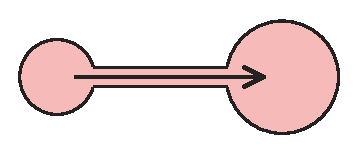
\includegraphics{GP013F10.eps}}
 \put(0,20){\makebox(0,0)[tl]{\parbox{125mm}{
Как видим, давление пропорционально кривизне. Если 2 пузыря соединить трубкой, то воздух потечет из маленького в большой!
}}}
 \end{picture}\\
 Если пузырь не круглый, а, например, эллиптический с радиусами кривизны $R_x$ и $R_y$, то давление в нем будет
  \begin{displaymath}
  \texttt{не }\hspace{10mm}\frac{2\,\alpha}R \;, \hspace{10mm}\texttt{ а } \hspace{10mm} p=\frac{\alpha}{R_x}+\frac{\alpha}{R_y}
  \end{displaymath}
 В частности, для цилиндрической поверхности один из радиусов = $\infty$, и давление в 2 раза меньше, чем для сферической:
  \begin{displaymath}
  p=\frac{\alpha}R \vspace*{2mm}
  \end{displaymath}

\underline{\bf Явления на границе жидкости и тв.тела} \\
Два варианта:
\begin{enumerate}
 \item молекулы жидкости притягиваются друг к другу сильнее, чем к мо\-ле\-ку\-лам твердой поверхности (не смачивается)
 \item жидкость сильнее взаимодействует с твердым телом (смачивается)
\end{enumerate}
\begin{picture}(185,30)(0,0)
 %\put(0,0){\framebox(185,30)[b]{}}
 \put(85,0){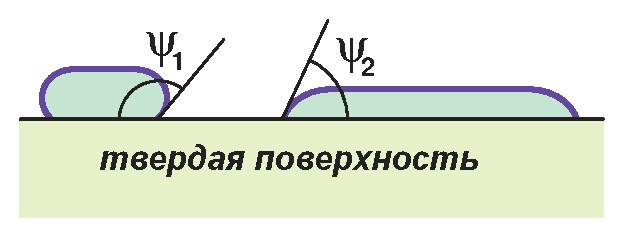
\includegraphics{GP013F11.eps}}
 \put(0,30){\makebox(0,0)[tl]{\parbox{80mm}{
{\bf краевой угол $\psi$}:
\begin{enumerate}
\item $\psi>\frac\pi2$ -- не смачивается
\item $\psi<\frac\pi2$ -- смачивается
\end{enumerate}
}}}
 \end{picture}\\
\begin{picture}(185,70)(0,0)
 %\put(0,0){\framebox(185,70)[b]{}}
 \put(0,0){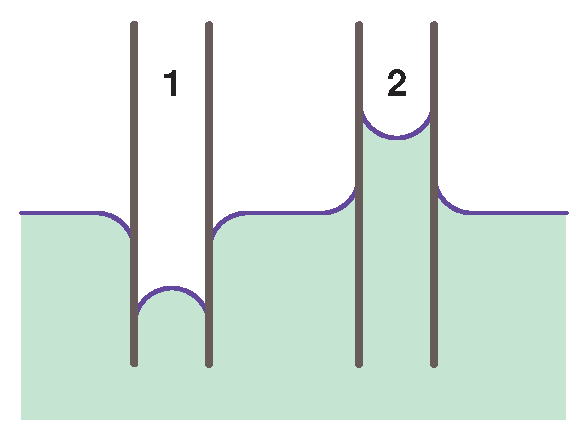
\includegraphics{GP013F12.eps}}
 \put(95,60){\makebox(0,0)[tl]{\parbox{90mm}{
Смачивается или нет -- зависит от веществ. Вода смачивает стекло, но не смачивает парафин. Ртуть не смачивает стекло, но смачивает железо, и т. д. Хорошо видно на капиллярах по {\bf форме мениска}. Перепад высот однозначно с этим связан (через краевой угол).
}}}
 \end{picture}\\
\begin{picture}(185,60)(0,0)
 %\put(0,0){\framebox(185,60)[b]{}}
 \put(130,0){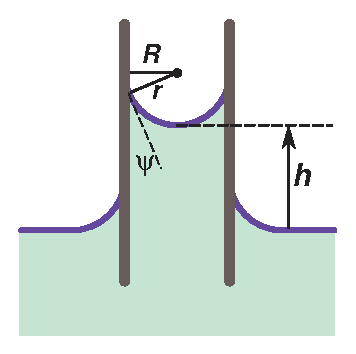
\includegraphics{GP013F13.eps}}
 \put(0,55){\makebox(0,0)[tl]{\parbox{140mm}{
 Давление столба жидкости высотой $h$ с плотностью $\rho$ должно уравновешиваться давлением, которое создает мениск с радиусом $r$:\vspace{-10mm}
 \begin{displaymath}
  \;\;\;\;\;\;\;p=\rho g h=\frac{2\alpha}r
 \end{displaymath}
}}}
 \put(0,25){\makebox(0,0)[tl]{\parbox{125mm}{
Поскольку радиус капилляра $R$ и радиус мениска $r$ связаны через краевой угол
($R=r\cos\psi$), то высоту $h$ можно отсюда определить как
}}}
 \end{picture}\vspace{-5mm}\\
 \begin{displaymath}
  h=\frac{2\alpha}{\rho g r}=\frac{2\alpha\cos\psi}{\rho g R}
 \end{displaymath}
Если смачиваемость 100\%-ная, то $\psi=0$, и $h\rightarrow \frac{2\alpha}{\rho g R}$. Если же сма\-чи\-ва\-е\-мость нулевая, то $\psi=2\pi$, $\cos\psi=-1$, и жидкость по капилляру не поднимается, а опускается.

Если надо измерить коэф-т поверхностного натяжения $\alpha$, то можно подобрать такой материал, который бы этой жидкостью или 100\% сма\-чи\-вал\-ся, или 100\% не смачивался, и просто замерить высоту.

Капиллярность: проникновение воды в почву и другие пористые материалы; фитили; флотация.\\
\begin{picture}(185,25)(0,0)
 %\put(0,0){\framebox(185,25)[b]{}}
 \put(103,0){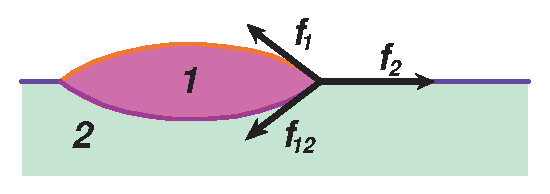
\includegraphics{GP013F14.eps}}
 \put(0,25){\makebox(0,0)[tl]{\parbox{98mm}{
 Если капля менее плотной жидкости растекается по более плотной, то
 $\exists$ 3 поверхностных натяжения: $\alpha_1$, $\alpha_2$ и $\alpha_{12}$
}}}
 \end{picture}\\
Силы $f_1$ и $f_{12}$ стягивают каплю, а сила $f_2$ заставляет ее растекаться. Равновесная форма капли -- когда все силы уравновешены. Это возможно при условии, что
\begin{displaymath}
 |\vec{f_2}|<|\vec{f_1}|+|\vec{f_{12}}|\hspace{10mm}\Rightarrow\hspace{10mm}
 \alpha_2<\alpha_1+\alpha_{12}
\end{displaymath}
Если же $\alpha_2$ намного больше, то капля будет растекаться бесконечно и образует мономолекулярный слой. Ленгмюр (Irving Langmuir, 1881-1957, N-Y; Нобелевская премия 1932 по химии за исследования поверхностных явлений) и Блоджетт (Katharine Blodgett, 1898-1979, N-Y). Метод при\-го\-тов\-ле\-ния мономолекулярных слоев.\\

\underline{\bf Испарение жидкостей}.\\
Находятся быстрые молекулы, которые преодолевают силы притяжения и, затрачивая на это преодоление некую часть энергии, вылетают из жидкости. Поскольку ее энергия при этом уменьшается, то жидкость охлаждается. Чтобы процесс шел изотермически, надо все время подводить тепло.

{\bf Удельная теплота испарения $\lambda$} -- кол-во тепла, которое надо сообщить ед-це массы жидкости, находящейся при температуре $T$, чтобы перевести ее в пар при той же температуре.   \\
$\lambda$ зависит от $T$: при $T\rightarrow T_k\;\;\lambda\rightarrow0$.\\

Если нагреть жидкость до такой $T$, при которой давление насыщенных паров = внешнему давлению, то испарение начинается не только с по\-верх\-но\-сти, но и по всему объему -- {\bf кипение}.\\

\underline{\bf Растворы}.\\
Рассмотрим слабый раствор, когда взаимодействием растворенных молекул между собой можно пренебречь. Они образуют как бы газ (отличие от идеального газа: движению мешают молекулы растворителя).

 Средняя кинетическая энергия: $\overline{w}=\frac12\,kT$ на степень свободы.
 Сово\-куп\-ность растворенных молекул должна оказывать {\bf осмотическое} да\-в\-ле\-ние $p=\frac23\,n_0\,\overline{w}$, и для них должно соблюдаться уравнение Менделеева-Кла\-пейрона:
 \begin{displaymath}
  pV=\frac m\mu RT
 \end{displaymath}
\begin{picture}(185,75)(0,0)
 %\put(0,0){\framebox(185,75)[b]{}}
 \put(155,0){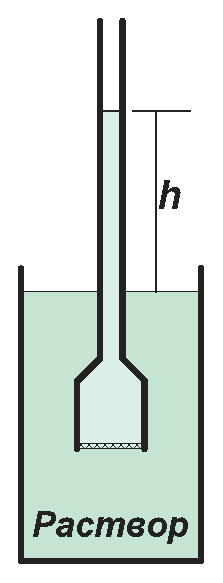
\includegraphics{GP013F15.eps}}
 \put(0,75){\makebox(0,0)[tl]{\parbox{150mm}{
 Если в растворе установить полупроницаемую мембрану (например, пропускающую воду, но не пропускающую растворенный в ней сахар), то сверху будет только давление воды, а снизу -- воды + сахара. Поэтому наверх будет проникать молекул воды больше, чем вниз, до тех пор, пока давление не уравновесится. Если равновесие наступило $\Rightarrow$ осмотическое (парциальное) давление сахара = дополнительному давлению столба воды $p=\rho\,g\,h$.
 Если обозначить концентрацию раствора как $C\equiv m/V$, то получаем \fbox{формулу Вант-Гоффа}:
}}}
 \end{picture}\\[-5mm]
 \begin{displaymath}
  p=\frac{C}\mu\, R\,T
 \end{displaymath}

 (Jacobus Henricus van 't Hoff, 1852-1911, Rotterdam; 1901 г.: Нобелевская премия по химии)

 При измерении осмотического давления для растворов разных веществ было найдено, что во многих случаях результаты согласуются с формулой Вант-Гоффа, но не всегда. Для растворов неорганических солей осмоти\-чес\-кое давление существенно БОЛЬШЕ. Причина: при растворении они диссоциируют на части, число частиц на единицу объема растворителя возрастает, а поскольку  $p=\frac23\,n_0\,\overline{w}$, то и осмотическое давление тоже возрастает.

 Те растворы, что подчиняются формуле Вант-Гоффа, -- не проводят эл.ток, а те, где $\exists$ диссоциация, -- проводят! Вывод: диссоциация идет не на АТОМЫ, а на ИОНЫ.
\end{document}
